% Primarily this section should be about scientific methods and theories you need to evaluate/compare/invent to solve your problems from 1.3.
% In some cases it may be ok to describe different technologies, but the purpose is to describe something and then draw a conclusion from that.
% Example, if you decide to discuss different databases, it may be for the purpose of selecting the best type for your implementation later on (based on for example data representation, scalability, speed, etc.).
% Optimally the problems in 1.3 are not solved by anyone else yet, in which case this section needs to describe how to solve them (new algorithms, mathematical approaches, etc.).
 
% This section can have a lot of subsections (3.1, 3.2, 3.3, etc).

% TODO: Explain Evaluation of values

The process of evaluating the value of a variableo or argument is a bit complicated because there is a lot of parts to it that all depend on each other.
Thus to simplify the explanation a simple example will be used to explain the main part of evaluatin the value.
Taking a look at the example in figure \ref{fig:subprogramexample} there is a function/subprogram die with the name \emph{my\_function}, it is the die with the tag \emph{DW\_TAG\_subprogram}.
The exmaple in the figure is the output of the program \emph{objdump} run on an \gls{DWARF} file and it is shown becuas it is much eaiser to read then the raw \gls{DWARF} file.
The function has a argument called \emph{val} which is the die with the tag \emph{DW\_TAG\_formal\_parameter} in the figure \ref{fig:subprogramexample}, it is a child of the function die which means that it is a argument to the function \emph{my\_function}.
It is this argument \emph{val} that will be used as an example for evaluatin the value of a variable or argument.
Examining the die for the argument \emph{val} there is a argument there called \emph{DW\_AT\_location} this arguments value is a number of operations that when executed will result in the location of the value.
In this example the value of the \emph{DW\_AT\_location} attribute is \emph{DW\_OP\_fbreg} $-2$, this operation means that the value is stored in memory at the address of the \emph{frame base} plust the offset $-2$(see \cite{dwarf} page 18).
\emph{Frame base} is a address in memory that is fixed to the first value in the stack for the funcitons stack frame(see \cite{dwarf} page 56).
To get the value of the \emph{frame base} it also has to be evaluated in the same way that the argument \emph{val} will be.
The operation for evaluationg the \emph{frame base} are located in the attribute \emph{DW\_AT\_frame\_base} in the parent function die called \emph{my\_function}.



\begin{figure}[h]
    \centering
    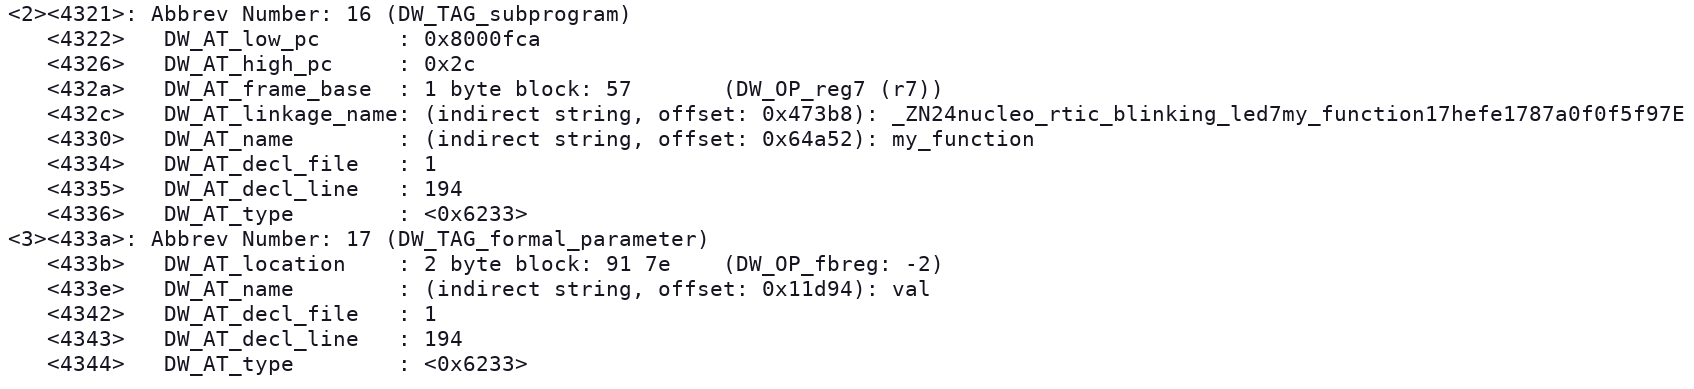
\includegraphics[width=1.0\textwidth]{subprogram-example.png}
    \label{fig:subprogramexample}
\end{figure}


\begin{figure}[h]
    \centering
    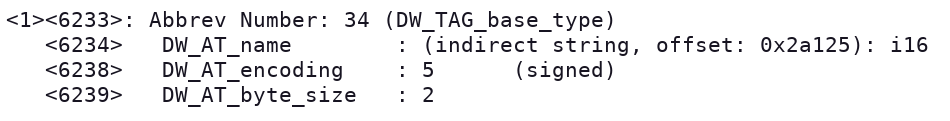
\includegraphics[width=1.0\textwidth]{basetype-example.png}
    \label{fig:basetypeexample}
\end{figure}

